\section{Reaction Forces}

\subsection{Types of Connections}

\begin{figure*}[!h]
\centering
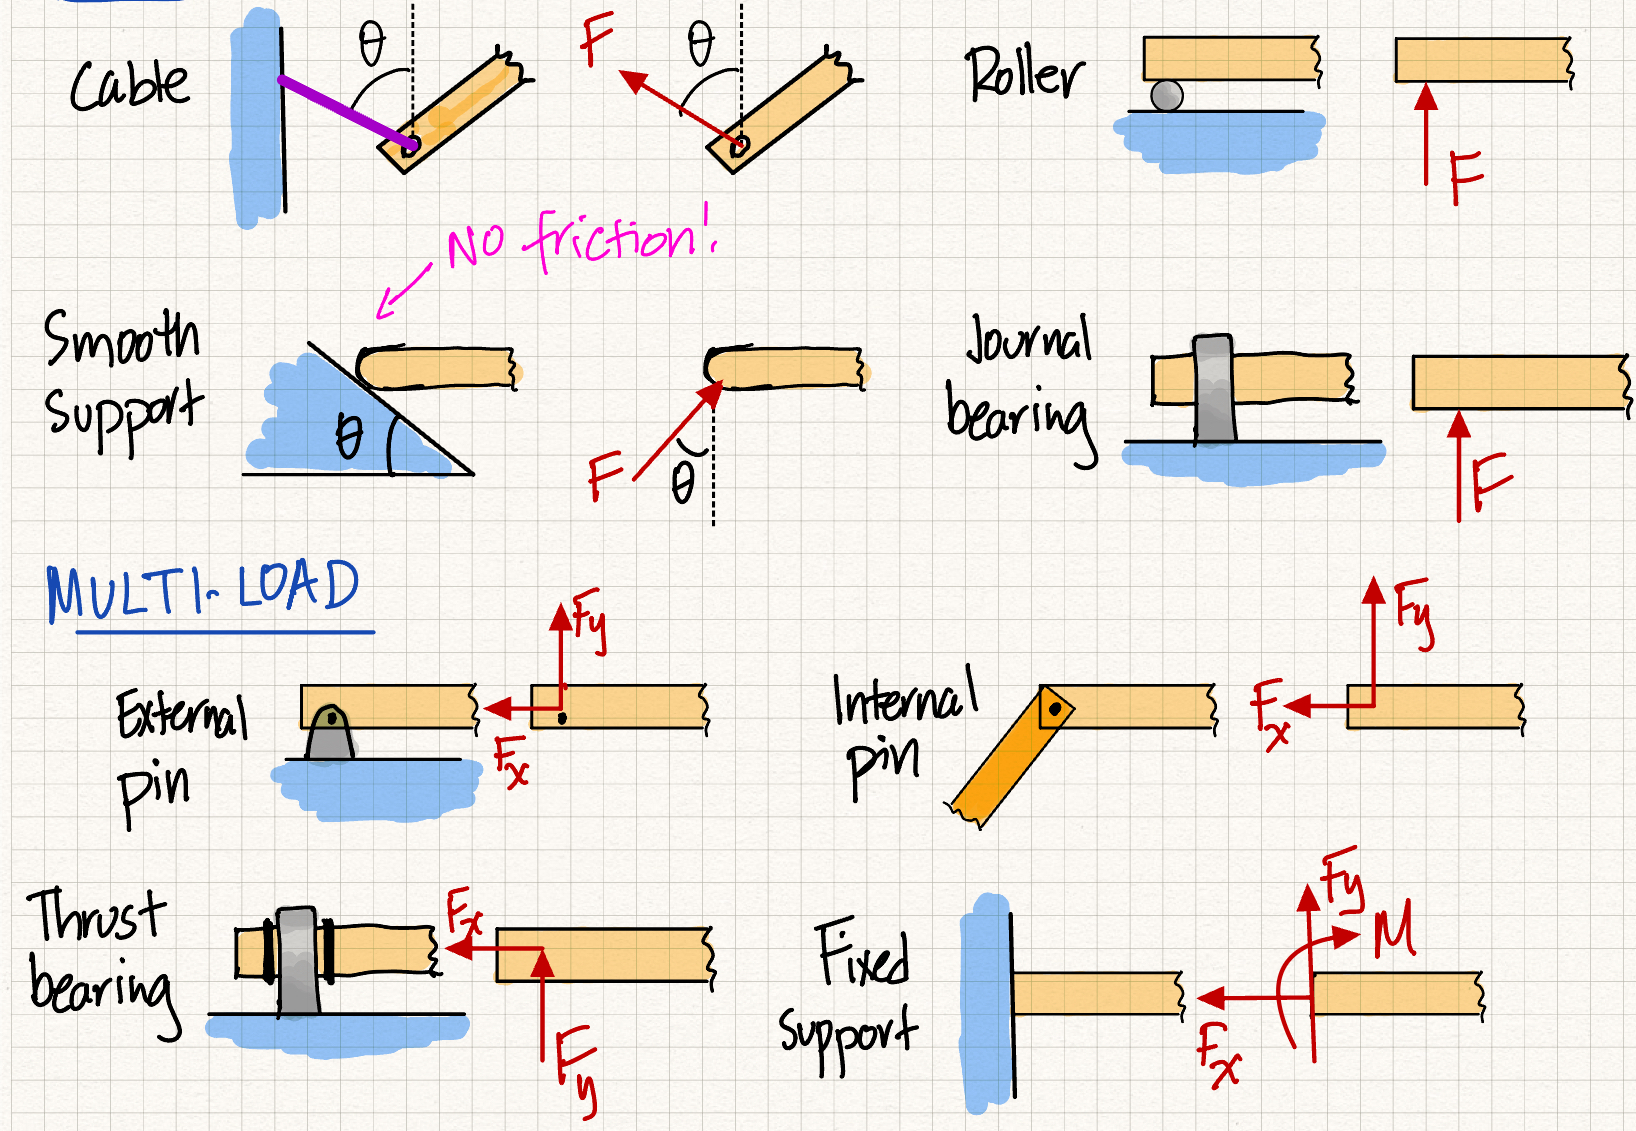
\includegraphics[angle=0, width=\textwidth]{ReactionForcesFigures/ReactionForces.jpg}
\vspace{-2mm}
\caption{\small \blue{Taken from Mariana Kersh's TAM 251 Lecture notes}}
\vspace{-3mm}
\label{Fig:NewtonsLaws}
\end{figure*}

\blue{Should we make a table for here? Some good examples of rigid constraints in real life in lecture 15.}

%From lecture 13

\blue{L13, Slide 3 had some good examples of support reactions if we want to make a pop up on the side eventually.}

\subsection{Redundant Constraints}

If a body has more supports than it needs to hold it in equilibrium, it is overly constrained. This will result in more unknown reaction forces than equations we can write, and the problem will not be solvable using statics alone. This type of system is a "statically indeterminate" system. 

%From lecture 15